\documentclass[14pt,a4paper]{article}
\usepackage[latin1]{inputenc}
\usepackage[T1]{fontenc}
\usepackage[english]{babel}
\usepackage{amsmath}
\usepackage{amsfonts}
\usepackage{amssymb}
\usepackage{makeidx}
\usepackage{amsthm}
\usepackage[margin=48pt]{geometry}
\usepackage[linesnumbered,ruled]{algorithm2e}
\usepackage{tikz}
\usetikzlibrary{automata, positioning}
\usepackage{float}
\usepackage[round]{natbib}
\usepackage[hidelinks]{hyperref}
\usepackage{caption}
\usepackage{graphicx}
\usepackage{subcaption}
\usepackage{listings}
\usepackage{color}
%\usepackage[justification=centering]{caption}


\makeatletter
\@addtoreset{section}{part}
\makeatother  


\let\oldpart\part
\renewcommand\part{\newpage\oldpart}

\def\code#1{\texttt{#1}}
\newtheorem{theorem}{Theorem}
\def\iff{\Leftrightarrow}
\theoremstyle{definition}
\newtheorem{madef}{Definition}
\newtheorem{prop}{Proposition}


 
\definecolor{codegreen}{rgb}{0,0.6,0}
\definecolor{codegray}{rgb}{0.5,0.5,0.5}
\definecolor{codepurple}{rgb}{0.58,0,0.82}
\definecolor{backcolour}{rgb}{0.95,0.95,0.92}

\lstdefinestyle{mystyle}{
    backgroundcolor=\color{backcolour},   
    commentstyle=\color{codegreen},
    keywordstyle=\color{magenta},
    numberstyle=\tiny\color{codegray},
    stringstyle=\color{codepurple},
    basicstyle=\footnotesize,
    breakatwhitespace=false,         
    breaklines=true,                 
    captionpos=b,                    
    keepspaces=true,                 
    numbers=left,                    
    numbersep=5pt,                  
    showspaces=false,                
    showstringspaces=false,
    showtabs=false,                  
    tabsize=2
}
 
\lstset{style=mystyle}



\oddsidemargin  0in
\evensidemargin  0in
\textwidth   6.3in
\textheight  9.5in
\topmargin  -0.7in


\usepackage{fancyhdr}
\pagestyle{fancy}
%\lfoot{Charles DUFOUR}
%\rfoot{\today}
\fancyhead[R]{}


\author{Charles Dufour}
\title{Bachelor Project: \\
Reinforcement learning and robot navigation}
\begin{document}

\begin{titlepage}
\newcommand{\HRule}{\rule{\linewidth}{0.5mm}} % Defines a new command for the horizontal lines, change thickness here

\center % Center everything on the page
 
%----------------------------------------------------------------------------------------
%   HEADING SECTIONS
%----------------------------------------------------------------------------------------

\vspace{3cm}
\textsc{\LARGE \'Ecole polytechnique f\'ed\'erale de Lausanne}\\[0.5cm] % Name of your university/college
\textsc{\large Disopt}\\[1.5cm] % Name of your university/college
\textsc{\LARGE Bachelor project}\\[0.5cm] % Major heading such as course name
\textsc{\large Spring Semester 2018 }\\[0.5cm] % Minor heading such as course title

%----------------------------------------------------------------------------------------
%   TITLE SECTION
%----------------------------------------------------------------------------------------

\HRule \\[0.4cm]
{ \huge \bfseries Reinforcement learning and robot navigation}\\[0.4cm] % Title of your document
\HRule \\[1.5cm]
 
%----------------------------------------------------------------------------------------
%   AUTHOR SECTION
%----------------------------------------------------------------------------------------

\begin{minipage}{0.4\textwidth}
\begin{flushleft} \large
\emph{Student:}\\
Charles Dufour
\end{flushleft}
\end{minipage}
~
\begin{minipage}{0.4\textwidth}
\begin{flushright} \large
\emph{Supervisors:} \\
Prof. Friedrich Eisenbrand \\% Supervisor's Name
Jonas Racine
\end{flushright}
\end{minipage}\\[5cm]

%----------------------------------------------------------------------------------------
%   LOGO SECTION
%----------------------------------------------------------------------------------------

 \includegraphics[width=0.5\linewidth]{img/logo_EPFL.eps}\\[1cm] % Include a department/university logo - this will require the graphicx package
 
%----------------------------------------------------------------------------------------

\vfill % Fill the rest of the page with whitespace

\end{titlepage}



%\begin{titlepage}
%   \vspace*{\stretch{1.0}}
%   \begin{center}
%      \Large\textbf{Reinforcement learning and robot navigation}\\
%      
%      \large\textbf{ }\\
%      \large\textit{Bachelor Project}
%   \end{center}
%   \vspace*{\stretch{2.0}}
%   
%   \vfill 
%   {\centering Charles Dufour, EPFL\par}
%\end{titlepage}

\newpage


\begin{abstract}

This dissertation focuses on the intelligent robot control in autonomous navigation using reinforcement learning. More precisely, the purpose of this bachelor project is to make a Raspberry Pi 3 powered robot adapt its behavior when facing a  traffic light using reinforcement learning, and more precisely Q-learning.We will first discuss the theory, then we will implement Q-learning on our robot, consider the results and then discuss further work. This project is the successor of many projects on the robot in  DISOPT. 

\nocite{Xia2015}
\nocite{KLMSurvey}
\end{abstract}
\vspace{0.5cm}


\tableofcontents
\pagenumbering{gobble}
\newpage
\fancyhead[L]{\emph{THEORY}}





\pagenumbering{arabic}
\section*{Introduction}

The purpose of this project is to apply reinforcement learning on the Raspberry Pi robot, specifically Q-learning algorithm. the robot is already able to follow lines on the ground using different techniques: support vector machine (SVM), proportional integral derivative (PID), neural networks \ldots 

The task was to make the robot adapt its behavior when facing a traffic light using the camera to detect the traffic light. We choose to use the technique using SVM to follow the line on the ground because even if it is one of the two techniques using the camera to follow the line (SVM, neural networks), it proved to be sufficiently smooth and reliable while light computationally speaking, in opposition to the neural network which was quite heavy and the PID which was not so smooth.\\


In this project we will first talk about the theory behind reinforcement learning in Part \ref{Theory}. Markov decision process, optimal policies and methods to compute them will be discussed in this part, and especially in Section \ref{TD}, we will talk about Q-learning algorithms.  The part before the Q-learning is necessary to understand why Q-learning algorithm works this way.

Then in Part \ref{Implementation}, we will talk about the implementation on the robot. We describe the modelization of our problem, and the difficulties we encountered.  We first try to use deep-learning to detect the traffic light with the camera, but it happens to be too slow for our robot: only one image per second was analyzed and we need more or less 10 per second so that the robot can follow the line. Hence we developed a home-made algorithm to detect the traffic light which is described in Subsection \ref{detection}. Then to efficiently learn, we had to learn through simulation and Section \ref{simulation} describe that. \\

Finally we present the results of our algorithm and possible further work.


\newpage
\part{Theory} \label{Theory}
\section{Reinforcement learning, a short introduction}

\begin{figure}[H]
\centering
\includegraphics[scale=0.5]{img/RL_graph.png}
\caption{Graphical representation of the reinforcement learning process from \citep{Sutton}}
\label{RL}
\end{figure}

In reinforcement learning problems, a scalar value, which we will call the reward, is received by an agent for transitions to one state to another. The aim of the agent is to maximize the discounted sum of the rewards he will receive, and to do so has to find an appropriate behavior (policy).


Our agent is connected to the model trough perceptions and actions. The typical procedure is as follows: 
\begin{itemize}
\item the environment sends an information to the agent about the state he is
\item then the agent chooses to do an action, based on the information he just received, the action takes him to another state in the environment
\item the environment sends back to the agent a reward (numerical signal, a single number) for the transition that just happened and also an information about the state the action brought our agent into
\item and so on $\ldots$
\end{itemize}

The purpose of our agent is to learn an optimal behavior which should optimize the long-run sum of values of the reinforcement signal (the rewards). \citep{KLMSurvey}

We define an \emph{episode} as being a finite sequence of event perceived by our agent (perception,action,reward,\ldots) The last state of an episode, the one that defines when it ends, is called an \emph{absorbing state}.

\section{MDP: Markov decision processes} \label{def_MDP}



The mathematical way to define the reinforcement learning framework is done using Markov decision processes.

Markov's decision processes are a tuple  $\mathcal{M}=\{\mathcal{S},\mathcal{A},T,R,\gamma\}$: 

\begin{itemize}
\item a set of states: $\mathcal{S}=\{s_0,s_1,\ldots,s_n\}$
\item a set of actions: $\mathcal{A}=\{a_1,a_2,\ldots ,a_k\}$
\item a transition function:  $T(s,a,s') \sim  Pr(s'\mid a, s) \quad s,s' \in \mathcal{S}$ which gives the state transition probabilities
\item a reward function: $R:\mathcal{S}\mapsto \mathbb{R} $
\item a discount factor $\gamma \in [0,1)$
\end{itemize}


The discount factor $\gamma $ helps making our learning agent more or less far-sighted: $\gamma$ can be interpreted as the relative importance it will give to future rewards compared to immediate ones.

$\mathcal{M}$ is a MDP if it respects the Markov property which is that the transitions only depends on the current state and action: 
\begin{equation*}
\mathbb{P}(s_{n+1}\mid a_{n+1},s_{n},a_{n},s_{n-1},\ldots)=\mathbb{P}(s_{n+1}\mid a_{n+1},s_{n})\\
\end{equation*}


When an agent is evolving in a MDP, what it observes is a sequence of states, actions and rewards: suppose the agent is in the state $s_0$ and chooses action $a_1$ and then end up in state $s_1$ with reward $r_1$; then the sequence observed is of the form: $s_0,a_1,s_1,r_1,a_2,s_2,r_2\ldots$


Markov decisions processes can easily be  represented as a directed graph: the nodes are the states and the directed edges from a node $Q$ are the actions an agent can choose to make while being in state $Q$, which will bring the agent in the state represented by the node at the endpoint of the edge as we can see in figure \ref{figure: graph_example}.


\begin{figure}[H]
\centering
\captionsetup{justification=centering,margin=2cm}
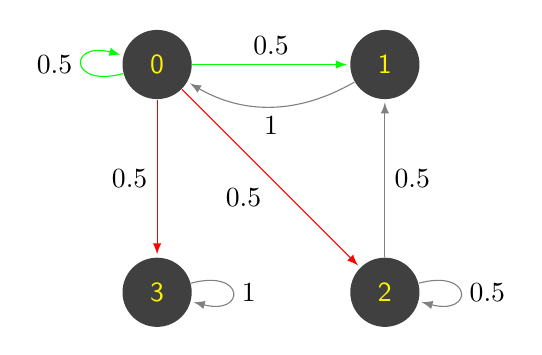
\begin{tikzpicture}[font=\sffamily]
    % Add the states
        \node[state,
              text=yellow,
              draw=none,
              fill=gray!50!black] (0) {0};
        \node[state,
              right=2cm of 0,
              text=yellow,
              draw=none, 
              fill=gray!50!black] (1) {1};
        \node[state,
              below=2cm of 1,
              text=yellow,
              draw=none, 
              fill=gray!50!black] (2) {2};
        \node[state,
        	  below = 2cm of 0,
        	  text=yellow,
        	  draw=none,
        	  fill=gray!50!black] (3) {3};
     

              
 \draw[every loop,
        auto=right,
        >=latex,
        draw=gray,
        fill=gray]
        
        	(0) edge[loop left, draw = green] node {$0.5$}(0)
        	(0) edge[ auto = right,draw = red]  node {$0.5$}(2)
        	(0) edge[auto = right,draw = red] node{$0.5$}  (3)
            (0) edge[auto = left,draw=green]  node {$0.5$} (1)
            (1) edge[bend left,auto =left]  node {$1$} (0)
            (2) edge[]  node {$0.5$}(1)
			(2) edge[loop right] node{$0.5$} (2)
			(3) edge[loop right] node{$1$} (3)	
			       
            ;       
      
    \end{tikzpicture}
    \caption{example of a graph representing a Markov Decision process, there are two actions possible from node $0$ which takes to different states with some probability }
     \label{figure: graph_example}
   
\end{figure}  




\section{Policies and Value functions}

A policy: $\pi $ is a stochastic mapping from states to actions: $$ \pi: \mathcal{A} \times \mathcal{S} \mapsto [0,1] \quad \text{s.t. } \sum_{a}\pi(a\mid s)=1 \quad \forall s \in \mathcal{S}$$
A policy is a formalization of the decision making process: in each state, we follow the policy to decide which action to choose with some probability. $\pi(a\mid s) $ is the probability that $A_{t+1}=a$ if $S_t=s$. Hence maximizing the reward means finding a good policy.


We need to quantify the reward the agent has to maximize, so we define the return as: 
$$G_t= r_{t+1}+\gamma r_{t+2}+ \dots = \sum_{k=0}^{\infty}\gamma^{k}r_{t+k+1} = r_{t+1} + \gamma G_{t+1} $$





Now we need a way to compare policy between them: for that we use the \emph{value functions}: the state value and the state-action value under a certain policy $\pi$. Intuitively they measure how good it is to be in a state (or respectively to take a specific action while being in a state) if we follow the policy afterwards.


Then we can define the value of taking action $a$ in state $s$ while following the policy $\pi$ as the expected return we would receive if we follow $\pi$:


\begin{equation*}
\begin{split}
v_{\pi}(s)&= \mathbb{E}_{\pi}[G_t \mid S_t=s]
\\&=\mathbb{E}_{\pi}\left[ r_{t+1} + \gamma G_{t+1} \mid S_t = s\right]
\\&=\mathbb{E}_{\pi}\left[ r_{t+1} \mid S_t = s \right] + \gamma \mathbb{E}_{\pi}\left[G_{t+1} \mid S_t = s \right]
\\&=\sum_{a}\pi(a \mid s)\sum_{s'}\mathbb{P}(s' \mid a,s)R(s') 
\\&+ \gamma \sum_{a}\pi(a \mid s)\sum_{s'}\mathbb{P}(s'\mid a,s)\mathbb{E}_{\pi}\left[G_{t+1} \mid S_{t+1} = s', S_{t}= s\right]
\end{split}
\end{equation*}

Using the Markovian property, $\mathbb{E}_{\pi}\left[G_{t+1} \mid S_{t+1}, S_{t}\right] = \mathbb{E}_{\pi}\left[G_{t+1} \mid S_{t+1}\right] $ so we get: 

\begin{equation}
\begin{split}
v_{\pi}(s)&= \sum_{a}\pi(a \mid s)\sum_{s'}\mathbb{P}(s'\mid a,s)\left[R(s') +\gamma \mathbb{E}_{\pi}\left[  G_{t+1} \mid S_{t+1}=s'  \right]\right]
\\&=\sum_{a}\pi(a \mid s)\sum_{s'}\mathbb{P}(s'\mid a,s)\left[R(s') + \gamma v_{\pi}(s')\right]
\end{split}
\label{v(s)}
\end{equation}



And the value of taking action $a$ while being in state $s$ under a policy $\pi$ following roughly the same method:

\begin{equation}
\begin{split}
q_{\pi}(s,a)&= \mathbb{E}\left[G_t\mid S_t=s, A_t=a\right]
\\&=\mathbb{E}\left[\sum_{k=0}^{\infty}\gamma^{k}r_{t+k+1}\mid S_t=s,A_t=a\right]
\\&= \sum_{s'}\mathbb{P}(s'\mid a,s)\left[R(s')+\gamma v_{\pi}(s')\right]
\end{split}
\label{q(s,a)}
\end{equation}



We can see from equations (\ref{v(s)}) and (\ref{q(s,a)})  that: 
\begin{equation}
v_{\pi}(s)=\sum_{a}\pi(a\mid s)q_{\pi}(s,a)
\end{equation}

These equations are called the Bellman equations and can be used to compute the value functions using dynamic programming, since they give recursive definition of the value functions.




\section{Optimal policies and Optimal value function}

In finite MDPs, the value function defines a partial order in the space of policies: 
$$ 
\pi\leq \pi' \iff v_{\pi} (s)\leq v_{\pi'} (s) \quad \forall s \in \mathcal{S}
$$

An optimal policy is a policy which is greater than or equal to any other policy. This is what we are interested in finding.

We can show that there is no policy strictly better than every deterministic policy \citep{Puterman} so there is always a deterministic optimal policy since there is only a finite number of deterministic policies.


We may have multiple optimal policies but they will all have the same value functions, as otherwise they would not be optimal policies with respect to the partial order define above. We denote these functions $q_{*}$ and $v_{*}$.

\paragraph{Bellman optimality equations}

The optimal policy must then takes the action that will be the more useful in term of rewards, i.e. having the best expected reward, otherwise updating the policy $\pi$ to a new policy $\pi'$ s.t.the policy $\pi'$ takes the best possible action in the state where $\pi$ does not, $\pi'$ would be better than $\pi$.

The optimal policy $\pi^*$ has  optimal value functions: $v_* $ and $ q_*$, which satisfy the following relations:

\begin{equation}
\begin{split}
v_{*}(s)&=\max_{a}q_{*}(s,a)
\\&=\max_{a} \sum_{s'}\mathbb{P}(s'\mid a,s)\left[R(s')+\gamma v_{*}(s')\right]
\end{split}
\label{bellman_opt_v}
\end{equation}

\begin{equation}
\begin{split}
q_{*}(s,a)&=\mathbb{E}\left[ R_{t+1} + \gamma v_{*}(S_ {t+1}) \mid S_t = s, A_t = a \right]
\\&=\mathbb{E}\left[ R_{t+1} + \gamma \max_{a'} q_{*}(S_{t+1},a') \mid S_t = s, A_t = a \right]
\\&= \sum_{s'}\mathbb{P}(s' \mid s,a)[R(s')+\gamma \max_{a'}q_{*}(s',a')]
\end{split}
\label{bellman_opt_q}
\end{equation}

These are called the \emph{Bellman optimality equations}. What equation (\ref{bellman_opt_v}) means intuitively is that the value of a state under $\pi^*$ must equal the expected return for the best action we can take from that state.


For finite MDPs these equations have a unique solution. We can show that if we know $v_{*}$ or $q_{*}$ a greedy approach to define a policy (best in the short term) becomes a long-term optimal solution. this is because defining a policy being greedy in function of $v_*$ implies that you go to the best state possible, the one with the biggest expected reward.


\section{Solving MDPs with dynamic programming}

In this section, we will assume we know the model of the environment (the transition function $\mathcal{T}$), and we will address the issue of computing efficiently approximation of the value functions, even if this is not what will be used in the implementation part, but it is necessary to understand the model-free algorithms as Q-learning, \ldots

From now on we assume our MDPs are finite, even if it is possible to extend everything to infinite MDPs if we are careful enough to avoid the problematic ones. \citep{Sutton}

One of the first method would be to scan the entire range of possible policies, then solve the Bellman optimality equations (\eqref{bellman_opt_q} and \eqref{bellman_opt_v}) for each policy and then compare them, but this would be less efficient as the following methods.

\subsection{Policy iteration}

This method uses two processes. The first one is policy evaluation where we compute the value function of a policy for all the states $s \in \mathcal{S} $; then we use the second one, policy improvement, to get a better policy by acting greedy. We describe them in details below.
\paragraph{Policy evaluation} 


We begin by setting arbitrary $v(s) \ \forall s \in \mathcal{S}$.
Then we update using one of the following update rules: 

\begin{itemize}
\item $v_{k+1}(s)=\underset{a \in A}{\sum}\pi(a \mid s)\underset{s'}{\sum}\mathbb{P}(s'\mid a,s)(R(s')+\gamma v_k(s'))$ \quad this is called "iterative policy evaluation".
\item we can use the same update rule as before, but use new information as soon as it is available. The algorithm would then be called in place due to this change.
\end{itemize}

From this we derive Algorithm \ref{algo1}.


\begin{algorithm}

    \SetKwInOut{Input}{Input}
    \SetKwInOut{Output}{Output}

    %\underline{function Euclid} $(a,b)$\;
    \Input{policy to evaluate $\pi$}
    \Output{$V \approx v_{\pi}$}
    Initialize $V = 0$\\
    \While{$\Delta \geq \varepsilon$}{
    	$\Delta = 0$\\
    	\For{$s\in \mathcal{S}$}{
    	 $v=V(s)$\\
    	 $V(s)=\underset{a}{\sum}\pi(a\mid s)\underset{s'}{\sum}\mathbb{P}(s'\mid a,s)[R(s')+\gamma V(s')]$\\
    	 $\Delta = \max(\Delta,\mid v-V(s)\mid)$\\
    	 }
       	}
       	\Return{$V \approx v_{\pi}$}
    
    \caption{Iterative policy evaluation (in place)}
    \label{algo1}
\end{algorithm}





\paragraph{Policy improvement}

We now find a better policy by computing whether we should change $a = \pi(s) $ to $ a'\neq\pi(s)$. In order to do so, we try to first select action $a'$ while being in state $s$ and then follow the policy. If the expected reward we get by making this choice is better than the one we get by simply following our policy, we should update $\pi(s):=a'$.

Mathematically speaking we compare the value of taking action $a$ while being in the state s, $q_{\pi}(s,a)$, to the value of $s$, $v_{\pi}(s)$, then update if needed.

The greedy update rule we use to improve our policy is the idea behind Algorithm \ref{algo2}: 

$$ 
\pi'(s)=\text{arg}\max_{a \in A}q_{\pi}(s,a)
$$

\begin{algorithm}
    \SetKwInOut{Input}{Input}
    \SetKwInOut{Output}{Output}

    %\underline{function Euclid} $(a,b)$\;
    \Input{policy to improve $\pi$}
    \Output{$\pi'$ s.t: $\pi' \geq \pi$ }
    \For{$s\in \mathcal{S}$}{
    	$\pi'(s)=\underset{a \in A}{\text{argmax }}q_{\pi}(s,a)$
    	}
       	\Return{$\pi'$}
    
    \caption{Policy improvement}
    \label{algo2}

\end{algorithm}



\paragraph{Policy Iteration} By combining the two processes described above, we can derive an algorithm to sweep through all our states and update our policy until the changes between each sweep are too small. This procedure can be represented graphically by Figure \ref{fig:Sutton}, and has two parameters, $\varepsilon$, being the stopping criterion in reference to $\Delta$, the difference of value function between two successive updates , and $\gamma$ as describe in Section \ref{def_MDP}.




\begin{figure}[ht]
\centering
\captionsetup{justification=centering,margin=2cm}

\includegraphics[scale=0.7]{img/policy_iter_sutton.PNG}
\caption{Graphical representation of the interactions between policy improvement and policy evaluation(from \citep{Sutton})}
\label{fig:Sutton}
\end{figure}






Algorithm \ref{algo3} terminates since there is only a finite number of deterministic policies.
The reason why  Algorithm~\ref{algo3} works is called the the \emph{policy improvement theorem}:

\begin{theorem}
Let $\pi$ and $\pi'$ be any pair of policies such that  $\forall s \in \mathcal{S}: $
\begin{equation}
q_{\pi'}(s,\pi'(s))\geq v_{\pi}(s) \label{th1}
\end{equation}
then:
\begin{equation}
\pi' \geq \pi \label{th2}
\end{equation}


Moreover if there is a strict inequality in all the states in \eqref{th1} then there must be at least a strict inequality for one state in \eqref{th2}
\end{theorem}


\begin{proof}
The idea of the proof is to expand the $q_{\pi}$ side until we get $v_{\pi'}(s)$ using Equation~\ref{q(s,a)} in page \pageref{q(s,a)}.

Indeed we have: 
\begin{equation}
\begin{split}
v_{\pi}(s) &\leq q_{\pi}(s,\pi'(s))
\\&=\mathbb{E}[r_{t+1}+\gamma v_{\pi}(S_{t+1})\mid S_{t}=s, A_{t}=\pi'(a)]
\\&=\mathbb{E}_{\pi'}[r_{t+1}+\gamma v_{\pi}(S_{t+1})\mid S_{t}=s]
\\& \leq \mathbb{E}_{\pi'}[r_{t+1}+\gamma q_{\pi}(S_{t+1},\pi'(S_{t+1}) \mid S_{t}=s]
\\& = \mathbb{E}_{\pi'}[r_{t+1}+\gamma \mathbb{E}_{\pi'}[r_{t+2}+\gamma v_{\pi}(S_{t+2})]\mid S_{t}=s]
\\& = \mathbb{E}_{\pi'}[r_{t+1}+\gamma r_{t+2}+\gamma^2 v_{\pi}(S_{t+2})\mid S_{t}=s]
\\& \leq \ldots
\\&= v_{\pi'}(s)
\end{split}
\end{equation}
\end{proof}


\begin{algorithm}
	\SetKwInOut{Input}{Input}
    \SetKwInOut{Output}{Output}
    
	\Input{arbitrary policy, stopping criterion $\varepsilon$}
	\Output{estimation of the optimal policy and of its value function}
	
	Policy evaluation:\\
	    \While{$\Delta \geq \varepsilon$}{
    	$\Delta = 0$\\
    	\For{$s\in \mathcal{S}$}{
    	 $v=V(s)$\\
    	 $V(s)=\underset{a}{\sum}\pi(a\mid s)\underset{s'}{\sum}\mathbb{P}(s'\mid a,s)[R(s')+\gamma V(s')]$\\
    	 $\Delta = \max(\Delta,\mid v-V(s)\mid)$\\
    	 }
       	}
     
     Policy improvement: \\
     policy-stable = true \\
     \For{$s \in \mathcal{S}$}{
     old-action= $\pi(s)$\\     
     $\pi(s)=\underset{a \in A}{\text{argmax}}q_{\pi}(s,a)$\\
     \If{old-action $\neq \pi(s)$}{
     policy-stable = false}
     }
     \eIf{policy-stable}{
     \Return{$V \approx v^{*} \text{and} \quad \pi \approx \pi^{*}$}
     }{Go to Policy evaluation}
     
	\caption{Policy Iteration}
	\label{algo3}
\end{algorithm}







\subsection{Other types of DP method}

\paragraph{Value Iteration}
Value iteration is another way of approximating an optimal policy. It combines improvement and evaluation in each of its sweep.

\begin{algorithm}[H]
	\SetKwInOut{Input}{Input}
    \SetKwInOut{Output}{Output}
    \label{algo4}
    
    \Input{policy}
    \Output{estimate of optimal policy}    
	    
    Initialize V arbitrarily 
    \While{$\Delta \geq \varepsilon$}{
    	$v=V(s)$\\
    	$V(s)=\underset{a}{\max}\underset{s'}{\sum}\mathbb{P}(s'\mid s,a)[R(s')+\gamma v_{k}(s')]$\\
    	$\Delta =\max(\Delta,\mid v-V(s) \mid)$\\    	
    }
    \Return{$\pi \approx \pi^{*}$ s.t: $\pi(s)=\underset{a}{\text{argmax}}\underset{s'}{\sum}\mathbb{P}(s'\mid s,a)[R(s')+\gamma v_{k}(s')]$}
    

    
\caption{Value iteration}
\end{algorithm}



\begin{theorem}
Algorithm \ref{algo4} finishes if the number of states is finite 
\end{theorem}

\begin{proof} 
We define the Bellman operator: $\mathcal{T}:\mathbb{R}^{\mid \mathcal{S}\mid } \mapsto \mathbb{R}^{\mid \mathcal{S}\mid }$ in the following way:
\begin{equation*}
(\mathcal{T}V)(s)=\max_{a \in \mathcal{A}}\sum_{s'}\mathbb{P}(s'\mid a,s)\left[ R(s') + \gamma V(s') \right]
\end{equation*}

In particular this operator is a contraction in the infinity norm, and hence our convergence problem is equivalent to the well known fixed point problem. we recall the inequality: 
\begin{equation}
\mid \max_{z}f(z)-\max_{z}h(z)\mid \leq \max_{z}\mid f(z) - h(z)\mid
\label{inter}
\end{equation}
and use it to develop: 
\begin{equation*}
\begin{split}
\mid \mathcal{T}V(s) - \mathcal{T}V'(s) \mid & \leq \mid \max_{a \in \mathcal{A}}\sum_{s'}\mathbb{P}(s'\mid a,s)\left[ R(s') + \gamma V(s') \right] - \max_{a \in \mathcal{A}}\sum_{s'}\mathbb{P}(s'\mid a,s)\left[ R(s') + \gamma V'(s') \right]\mid
\\& \stackrel{(\ref{inter})}{\leq} \max_{a \in \mathcal{A}}\mid \sum_{s'}\mathbb{P}(s'\mid a,s)\left[ R(s') + \gamma V(s') \right] - \sum_{s'}\mathbb{P}(s'\mid a,s)\left[ R(s') + \gamma V'(s') \right]\mid
\\&\leq \max _{a}\gamma \mid \sum_{s'}\mathbb{P}(s'\mid a,s)\left[ V(s')-V'(s')\right] \mid
\\& \leq \gamma \max_{s} \mid V(s)-V'(s) \mid
\\& \leq \gamma \mid \mid V-V'\mid \mid _{\infty}
\end{split}
\end{equation*}

Now using the property that a contraction has a unique fixed point and that all sequences $V,\mathcal{T}V,\mathcal{T}^2V,\ldots $ converges towards this fixed point we get the convergence.


\end{proof}

\subsection{Other methods}



There exists some others dynamic programming algorithm to solve these problems: 
\begin{itemize}
\item Asynchronous Dynamic programming: it doe not sweep amongst all the states at each iteration. They are in place iterative DP algorithms.
\item General Policy Iteration (GPI): they are mixing the two components of policy iteration (evaluation and improvement) a little bit more than the algorithm we already saw.
\end{itemize}

The most important drawback to these methods is that they are model-based, meaning that we need to have a complete knowledge of the model (the transition function) to implement those.

\section{Model-free approaches and algorithms}

Until now, we assumed implicitly that we knew the model (i.e. the transition function) of our environment and all the previous learning algorithms were based on this assumption. Hence we call them \emph{model-based},and we can not apply them without knowing the model. But in real life applications, we often do not know the whole model, and we have to study other methods in order to do reinforcement learning,which we call \emph{model-free} algorithms. We will discuss shortly some of them in this section, then introduce Q-learning algorithms and then proceed to the implementation part.


\subsection{exploration exploitation dilemma}

When the agent learn from experience, as when using model-free algorithm, it has to choose actions, then execute them and look at the reward from the environment in order to approximate the value functions (in Q-learning for example, we will try to approximate $q_\pi(s,a)$). To choose the actions, the agent has two choices:
\begin{itemize}
\item choose an action which is known already has having a good action value and improve this approximation. This is called exploitation.
\item try another action so maybe the agent will discover a better way to do its task. This is called exploration. 
\end{itemize}

For the agent to explore all states in order to have a good idea of what policy is the best, it is necessary that it explores the maximum number of states possible, but at the same time, it should constantly improve its approximations. This is the exploration exploitation dilemma, exploitation is useful to improve our estimates, but exploration is needed since there is always uncertainty about the accuracy of the present estimate, some actions may actually be better than our actual best ones. Efficient exploration of the action and state space is a crucial factor in the convergence rate of a learning scheme.

To solve this dilemma, we can use different techniques that will balance exploitation and exploration:
\begin{itemize}
\item random selection of action.
 \item $\varepsilon$-greedy manner: with probability $1-\varepsilon$ we choose exploitation, hence we take the best action we can, and otherwise we take another action at random between the ones possible and explore.
 \item UCB (Upper confidence bound) action selection: we choose action deterministically, but perform exploration by choosing the actions that have been tried the least.
 \item \ldots
\end{itemize}

In the $\varepsilon$-greedy approach, there are different ways to modify the $\varepsilon$ during the learning process: either we keep the same $\varepsilon$, or we good greedy in the limit. This produces the following definition: 

\begin{madef}
A policy is GLIE (Greedy in the limit with infinite exploration) if it respects the following properties:
\begin{itemize}
\item if a state is visited infinitely often then each action possible from this state is chosen infinitely often almost surely.
\item in the limit of number of episodes, the policy is greedy with respect to the action value approximated $q(s,a)$ 
\end{itemize}
\end{madef}

\subsection{Monte-Carlo methods}
Monte-Carlo methods use sampling from episodes to estimate the action value function.
They differ from the dynamic programming methods by the fact that they do not require a knowledge of the model to estimate the action value function of a policy. To improve our policy, we still use the same greedy approach as before, choosing the best actions available in each state.
Monte-Carlo methods estimate the value function by averaging the sample return from the episodes. Thus they only need sample sequences of state, action, reward from experience or simulation. \citep{Sutton}


 It can be shown to converge as long as all pairs $(s,a)$ with $s$ a state, and $a$ an action are visited an infinite number of time.
\subsection{Temporal difference methods} \label{TD}
Temporal difference methods are a combination of dynamic programming and Monte-Carlo methods. Unlike Monte Carlo methods, TD learning methods do not have to wait until an estimate of the return is available (i.e., at the end of an episode) to update the value function. Instead, they use temporal errors and only have to wait until the next time step. The temporal error is the difference between the old estimate and a new estimate of
the value function, taking into account the reward received in the current sample.
These updates are done iteratively and, in contrast to dynamic programming
methods, only take into account the sampled following states. \citep{Xia2015}

In this project the purpose is to implement Q-learning, which is a class of algorithm.


\paragraph{Q-learning} Estimation of the optimal action value function $q_*$ given in Equation (\ref{bellman_opt_q}):


with $s'$ the state resulting from action a:
\begin{equation}
Q(s,a) \leftarrow Q(s,a) + \alpha \left( \mathcal{R}(s') + \gamma \max_{a'}Q(s',a') - Q(s,a) \right) 
\label{eq:ql}
\end{equation}

Where $\alpha$ is the learning factor.  This factor determine in what extend do the newly obtained information overwrite the previous one. Even if the learning can fluctuate through the learning, often in practice the constant learning rate $\alpha = 0.1$ is considered since it respects the hypothesis of Theorem \ref{conv_theorem} and is easy to implement.

The Q-learning algorithms being iterative algorithm, they suppose an initial value. If the initial value is high, "optimistic initial conditions", this will encourage exploration. The updated action value will be lower than the initial value, and hence the explored action will be less likely to be chosen the next time we are in this state.

The actions are chosen so that we balance the exploration exploitation issue (random, greedy in the limit (GLIE),\ldots). \emph{Episode} in algorithm \ref{Ql:algo} is a list of episodes, one episode $\mathcal{E}$ being a finite successions of transitions  $<s,a,r,s'>$



\begin{theorem} (convergence of Q-learning algorithm)

As long as each pairs $(s,a)$ are visited infinitely many times, that $s'\sim T(s,a,s')$, $r \sim \mathcal{R}(s')$ and  $\underset{n \in \mathbb{N}}{\sum} \alpha = \infty$, $\underset{n \in \mathbb{N}}{\sum} \alpha^2 < \infty$, the Q-learning algorithm \ref{Ql:algo} converges.

\label{conv_theorem}
\end{theorem}

\begin{proof} 


See \citep{Watkins_article}

\end{proof}

\begin{algorithm}
	\SetKwInOut{Input}{Input}
    \SetKwInOut{Output}{Output}
    
	\Input{Q initialized at $0$, learning rate $\alpha$, discount factor $gamma$, exploration parameter $\varepsilon$, Episodes}
	\Output{estimation of the optimal value function $Q$ and optimal policy $\pi$}
	
	Approximation of the value function
	    \For{$\mathcal{E}$ in Episodes}{
    		\For{ $<s,a,r,s'>\quad \in \mathcal{E}$}{
    	 $Q(s,a) \leftarrow Q(s,a) + \alpha \left( \mathcal{R}(s') + \gamma \max_{a'}Q(s',a') - Q(s,a) \right)$
    	 }
       	}
     
     Policy: \\
     \For{$s \in \mathcal{S}$}{
     	$\pi(s)=\underset{a \in A}{\text{argmax}} ~Q(s,a)$\\
     }
     
	\caption{Q-learning algorithm}
	\label{Ql:algo}
\end{algorithm}

\newpage


\part{Implementation} \label{Implementation}
\fancyhead[L]{\emph{IMPLEMENTATION}}
%We have to determine our states, and hence a way for the robot to find its relative distance to our traffic light.
\section{The robot}
The robot is a Raspberry Pi 3 powered robot with a camera, as in Figure (\ref{fig:sub1}), and it follows a black line on the floor. On the right of this line, we put a \emph{traffic light}, in the form of a phone displaying a site that contains the traffic light animation (\url{http://light.grathink.com})  which is as one can see in Figure \ref{vue_robot}. The position of the activated region of the traffic light indicates the color: down is green, \ldots

\begin{figure}[H]
\centering
\begin{subfigure}{.5\textwidth}
  \centering
  \includegraphics[width=.5\linewidth]{img/robot.png}
  \caption{The raspberry pi 3 powered robot with one camera}
  \label{fig:sub1}
\end{subfigure}%
\begin{subfigure}{.5\textwidth}
  \centering
  \includegraphics[width=.5\linewidth]{img/setting1_mod1.png}
  \caption{The setting}
  \label{fig:sub2}
\end{subfigure}
\caption{The Framework of our runs}
\label{fig:test}
\end{figure}



\section{The task}
The robot can already follow lines from previous projects on it, and we want to learn how to respect a traffic light using reinforcement learning. In this project the robot is only allowed to go forward or to stop, but cannot go backwards.

The setting we have is represented in Figure \ref{fig:sub2}. The robot is placed at a distance of approximately 2 meters from the traffic light, follows a straight line and go forward.
The robot has a stopping zone a little bit before the traffic light where it should stop if the traffic light is red, and then restart when the traffic light changes from red.



\section{Modelization}

\subsection{States}
The states are modeled in the following way. In one state we have to have the information about
\begin{itemize}
\item   the distance to the traffic light.
\item the speed of the robot.
\item the color of the traffic light .
\item the "time spent in this color": how long has the robot been seeing the traffic light in the same color? This question helps us adapt more easily as a real driver would do. If we are driving a car and the traffic light is orange, depending for how long it has been in this state, we may speed up in order to pass before it turns to red.
\item the previous action. This is needed as way to try to control the smoothness of the driving and penalize chaotic driving. It is explained in details in subsection \ref{reward function}.

 \end{itemize}

One can represent the states in the following way: we have a graph like the one in Figure  \ref{figure: graph_example} for each speed, for example in Figure~\ref{figure: graph_ex}. Then we add as a second layer the information about the traffic light color, then a next one for the time spent in the color, and finally one for the action that brought the agent in this position.
\begin{figure}[H]
\begin{center}
    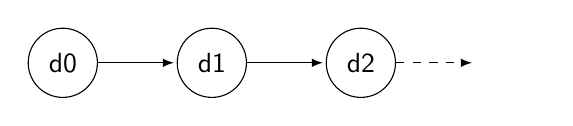
\begin{tikzpicture}[font=\sffamily]
    % Add the states
        \node[state,text=black] (d0) {d0};    
        \node[state,right = 1cm of d0,text=black] (d1) {d1};
        \node[state,right = 1cm of d1,text=black] (d2) {d2};
        \node[state,right = 1cm of d2,text=black,draw=none] (d3) {};       
              
        % Connect the states with arrows
        \draw[every loop,auto=right,>=latex,draw=black,fill=black]
        	(d0) edge[] (d1)
        	(d1) edge[] (d2)
        	(d2) edge[dashed] (d3)
            ;
    \end{tikzpicture}
\end{center}
    \caption{Exemple of a transition graph for a certain speed}
    \label{figure: graph_ex}

\end{figure}


The robot can go from speed $20$ to speed $100$  and we decided to consider the speeds $0,20,30,30,40,\ldots, 70$ for simplicity and we stopped at $70$ since if the robot goes faster, it has trouble following the line, and the distance detection becomes not reliable as Figure \ref{fig:mean and std of net44} shows.

\subsection{Detection of state} \label{detection}

The speed of the robot is easily obtained, and the rest of the information in order to decide in which state we are are obtained as explained below.

The distance to the traffic light is computed in the following way. The robot perceives images as represented in Figure \ref{vue_robot} and the algorithm for the image processing is done in the following way. We are going to compute the position of 
\begin{itemize}
\item a search zone if we have at least analyzed two images.
\item specific features that allow us to detect the phone: in particular this is the bright white pixels displayed at the top of the traffic light animation on the phone, there are represented in Figure \ref{vue_robot} as the phone detection points.
\item a reference point used to determine the distance to the traffic light, which is the bottom of the phone.
\item three sample points between the reference point and the detection points, they will allow us to identify which color is the traffic light on depending on their activation.
\end{itemize}

\begin{figure}[ht]
        \centering
        \captionsetup{justification=centering,margin=2cm}

        \begin{subfigure}[b]{0.49\textwidth}
            \centering
            \includegraphics[width=\textwidth]{img/vue7.png}   
            \label{fig:mean and std of net14}
        \end{subfigure}
        \begin{subfigure}[b]{0.49\textwidth}  
            \centering 
            \includegraphics[width=\textwidth]{img/vue10.png}
            \label{fig:mean and std of net24}
        \end{subfigure}
        \vskip\baselineskip
        
        \begin{subfigure}[b]{0.49\textwidth}   
            \centering 
            \includegraphics[width=\textwidth]{img/vue46.png}
   
            \label{fig:mean and std of net34}
        \end{subfigure}
        \begin{subfigure}[b]{0.49\textwidth}   
            \centering 
            \includegraphics[width=\textwidth]{img/vue51.png}
  
            \label{fig:mean and std of net44}
        \end{subfigure}
        \caption{{\small View from the robot's camera in our setting}}
	\label{vue_robot}
\end{figure}

In order to compute the positions of the specific points mentioned above, we will use the following procedure: 
\begin{itemize}
\item Scan the searching area for bright white pixels if there is a searching area, otherwise scan the whole left half of the image.
\item Find the middle of the zone of the white pixels
\item  From there go down to the bottom of the traffic light (end is detected as a value in all the RGB channel big enough)
\item distance = the number of pixels from the top of the image to the bottom of the traffic light
\item take three equidistant points between the zone with bright white pixels and the reference point.
 \item color is determined from the intensity of the different RGB channel in the sample points  
\end{itemize}

The distance is computed as the distance of the reference point in pixels. The detection had to happened fast so that the robot could still follow the line while analyzing our image; in order to do so, we refine our search area of the interesting features in a picture based on the previous distances computed. On Figure \ref{vue_robot}, we can see the evolution of the search zone.


\begin{figure}[h]
        \centering
        \begin{subfigure}[b]{0.475\textwidth}
            \centering
            \includegraphics[width=\textwidth]{img/dist30.png}
            \caption[Speed 30]%
            {{\small Speed 30}}    
            \label{fig:mean and std of net14}
        \end{subfigure}
        \hfill
        \begin{subfigure}[b]{0.475\textwidth}  
            \centering 
            \includegraphics[width=\textwidth]{img/dist50.png}
            \caption[]%
            {{\small Speed 50}}
            \label{fig:mean and std of net24}
        \end{subfigure}
        \vskip\baselineskip
        \begin{subfigure}[b]{0.475\textwidth}   
            \centering 
            \includegraphics[width=\textwidth]{img/dist70.png}
            \caption[]%
            {{\small Speed 70}}    
            \label{fig:mean and std of net34}
        \end{subfigure}
        \quad
        \begin{subfigure}[b]{0.475\textwidth}   
            \centering 
            \includegraphics[width=\textwidth]{img/dist100.png}
            \caption[]%
            {{\small Speed 100}}    
            \label{fig:mean and std of net44}
        \end{subfigure}
        \caption{{\small Evolution of the perceived distance at different speed}}
	\label{distance_plots}
\end{figure}


Now our robot has a way to perceives in which state he is. What actions can he take ? 


\subsection{Actions}
The action we are interested in do not concern the direction, which is imposed from the line on the ground as we can see from Figure (\ref{fig:sub2}). Hence we are only interested in accelerating or slowing down. The possible actions are the following:
\begin{itemize}
\item speed up which brings you in a speed higher (i.e. you go from $20$ to $30$) as can be seen in Figure \ref{acceleration} in a simplified model. If the robot has speed $70$ and accelerate, nothing happens.
\item keeping the same speed, which does not influence the speed.
\item slowing down, which work the opposite way of speeding up, except that slowing down while having speed $0$ does not have any effect.
\end{itemize}
The transitions from speed to "neighboring" speed is done in order to simulate smooth driving.
 The transitions from speed to speed can be seen as in Figure \ref{acceleration}, where the model is simplified. We only show 3 speeds, the acceleration action and the action of keeping the same speed.
\begin{figure}[ht]
\captionsetup{justification=centering,margin=2cm}
\begin{center}
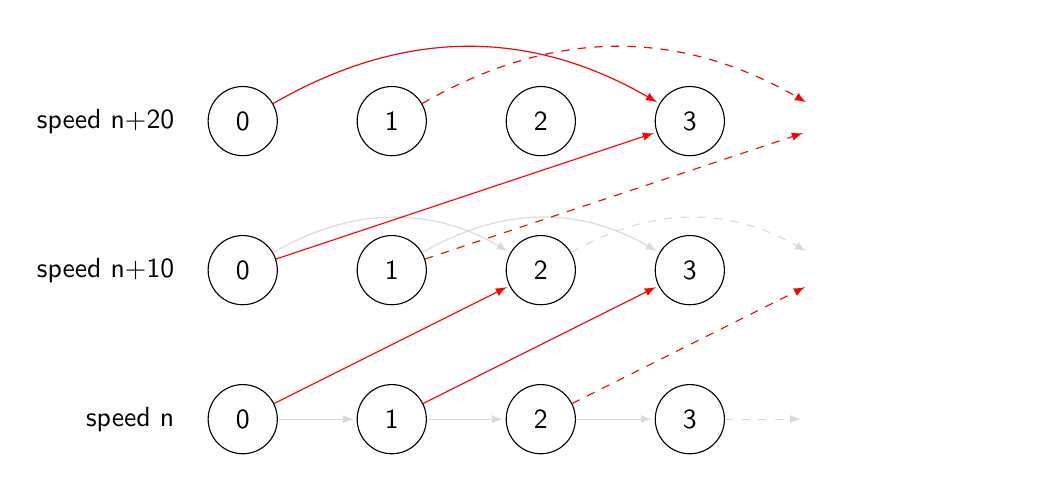
\begin{tikzpicture}[font=\sffamily]
    % Add the states
        %\node[state,draw=none] (d1) [left of=1] {};
        \node[state,text = black
              ] (h0) {0};
		\node[state,
			below=1 cm of h0,
			text = black
        	] (m0) {0};
		\node[state,
			below= 1 cm of m0,
        	text=black,
        	] (l0) {0};
         \node[state,
         	 right = 1 cm of h0,
             text = black
              ] (h1) {1};	
		\node[state,
			below=1 cm of h1,
        	text = black
        	] (m1) {1};
		\node[state,
			below= 1 cm of m1,
        	text=black,
        	] (l1) {1};
         \node[state,
         	right = 1 cm of h1,
         	text = black
              ] (h2) {2};	
		\node[state,
			below=1 cm of h2,
        	text = black,
        	] (m2) {2};
		\node[state,
		below= 1 cm of m2,
        	text=black,
        	] (l2) {2};
        \node[state,
        	right = 1 cm of h2,
        	text = black
             ] (h3) {3};	
		\node[state,
			below=1 cm of h3,
        	text=black
        	] (m3) {3};
		\node[state,
			below= 1 cm of m3,
        	text=black,
        	] (l3) {3};   	
		\node[state,draw=none] (d1) [right = 1 cm of l3] {};	
		\node[state,draw=none] (d2) [right = 1 cm of m3] {};
		\node[state,draw=none] (d3) [right = 1 cm of h3] {};
		\node[state,draw=none] (d4) [right = 1 cm of d3] {};
		\node[draw=none] (legend1) [left=0.3 cm of l0] {speed n};
		\node[draw=none] (legend2) [left = 0.3 cm of m0] {\textcolor{black}{speed n+10}};
		\node[draw=none] (legend3) [left = 0.3 cm of h0] {\textcolor{black}{speed n+20}};
		        
       \draw[every loop,
        auto=right,
        >=latex,
        draw=gray!30,
        fill=gray!30]
			(l0) edge[](l1)
			(l1) edge[] (l2)	
			(l2) edge[] (l3)
			(l3) edge[dashed] (d1)
			(m0) edge[bend left] (m2)
			(m1) edge[bend left] (m3)
			(m2) edge[bend left,dashed] (d2)
			(h0) edge[bend left] (h3)
			(h1) edge[bend left,dashed] (d3)
            ;
      \draw[every loop,
        auto=right,
        >=latex,
        draw=red,
        fill=red]
			(l0) edge[](m2)
			(l1) edge[] (m3)	
			(m0) edge[] (h3)
			(h0) edge[bend left] (h3)
			(h1) edge[bend left,dashed] (d3)
			(l2) edge[dashed] (d2)
			(m1) edge[dashed] (d3);
	\end{tikzpicture}
	\caption{graph representing some transitions (accelerating in red and keeping the same speed in light grey) in a simpler model of our environment: there are only 3 speeds}
    	\label{acceleration}
     \end{center}
\end{figure}

\subsection{Reward function} \label{reward function}

The reward function is defined so that the robot would go forward toward the traffic light, but adapts its speed with respect to the traffic light. In order to do that, we define all the states in which the position is after the traffic light as absorbing state: we do not consider how to behave once we have passed the traffic light or what to do when there is none, this can be easily coded and is not the purpose of this project.

The reward function used here is the one given by $\mathcal{R}(s,a)$, which means it takes into account the action we just did.

In order to define the reward function, we have to take a look at the behavior we want to make the robot learn: 
\begin{itemize}
\item If the robot plows through a red light, it should get a negative reward, but if it stops in front of a red light it should get a positive one.
\item If the robot stops when the traffic light is not red, it should get a negative reward and a positive for the opposite action.
\item If the actions following one another are inconsistent with each other (hits the brakes then goes full speed for example), we will give a negative reward whatever the position, as long as it is not an absorbing position. This is why we use the form of the reward function given before.
\end{itemize}

The reward function is actually really sensitive: if the relative importance of the rewards given for a certain transitions is slightly changed, this can completely modify the behavior of the agent. The actual code used for the reward function can be found in Annexe \ref{code}.

The robot has a designated "stopping zone" where it should respect the traffic light. If the robot is at a distance $50$ pixels of the traffic light, the detection of the traffic light is not accurate anymore, so we define this distance as the stop line there is on the ground in front of real traffic lights.

Then the robot is allowed to stop a little bit before the stopping line, as a real driver could do without problems. Hence this stopping zone begins at a distance of 10 pixels before the stopping line, distance obtained from experience (this is the smaller distance that yielded good results for respecting traffic light).




The precise parameters of the reward function where given by the results from experience, the one we used can be seen in the appendix \ref{code}.

\section{Simulation of the model} \label{simulation}

One can apply Q-learning on a modelization of the problem. We do not have to have the robot running around into walls to learn; if we can have a simulation of our problem, we could run everything in a simulated world and after that actually transfer the results to the robot directly.

In order to do that, we had to actually simulate the environment of the robot, i.e. the transition function in the definition of Markov decision processes (see Section (\ref{def_MDP})).


We decomposed the simulation in multiple parts: 
\begin{itemize}
\item at a given speed we needed to know the evolution of our newly defined distance. This gave data as can be seen in Figure \ref{distance_plots}, the framework is described in Appendix \ref{pictures}. But even with a lot of data sampling, we were not able to completely define the transitions, some portions were still missing. In order to solve this issue, we used an imputation process like \emph{hot deck}: when a datum was missing, it was imputed using information from the nearest data (if in a certain position there were no data, we used the information given by positions close to this one, computed a median of the data from these distances and then imputed it with a little noise).

 We then computed probability of transition from one position to another while being at a certain speed.
\item we need to know the transitions of the color of the traffic light. In order to do that we measured what was the speed of the image processing, in order to know how many images the robot processes in average in one second. From these data, we coded a traffic light that simulated a real one with the following time (in seconds): green $5$, orange $2$, red $3$, orange $2$, \ldots
\item the transitions between speeds are supposed deterministic, we do not account for any problems in the connection of the pins of the robot. But one can note that the transitions are in such way that if you decide to slow down while already in the lowest speed, you just stay in low speed, and the same phenomena happens while accelerating in the highest possible speed.
\end{itemize}

Then, having a simulation of our model, we are able to make our robot learn on it.



\section{Q-learning implementation}


We apply the Q-learning algorithm described in Equation (\ref{eq:ql}), with parameters $\alpha = 0.1$ and $\gamma = 0.9$ since they are the most common parameter in use for reinforcement learning and they respect the condition of Theorem \ref{conv_theorem}. The $\varepsilon$ parameter for balancing exploration and exploitation is decreasing from $0.1$ to $0$ linearly as we learn (decayed $\varepsilon$ or greedy in the limit (GLIE)). We learn over $5$ millions of episodes, one episode consisting on starting in front of a traffic light and stopping when we went passed a certain stopping distance from the traffic light (distance is linked to the fact that passed a certain point the camera of the robot does not see the light anymore).


\begin{figure}[h]
\centering
\captionsetup{justification=centering,margin=2cm}
\includegraphics[scale=0.6]{img/Q_learning_10m.png}
\caption{learning curve of the Q-learning algorithm \ref{Ql:algo} applied to our problem, $10$ million iterations}
\label{curve}
\end{figure}

We can verify how well the robot learns by visualizing the trajectory it would do: in Figure (\ref{trajectories}), we have the distance from the traffic light in the x axis , and on the y axis we have the speed. On the bottom of the graph we have the color the traffic light has during the run (the yellow color is representing the orange that comes after the red in the traffic light sequence): if there is a "pile" of points, it means the traffic light changed multiple times during the moment the robot was on this position. The robot is set to have a beginning distance of $200$ for data management purpose, so we can identify the beginning of a new episode from an error in the distance computation; that is why at the beginning of the trajectories there is this strange behavior of going from $200$ to about $125$ in a single shot, hence we did not show in the trajectories plot as in Figure \ref{trajectories} the first part of the graph since it was not relevant to the presentation of results or to interpretation of them.

From Figure \ref{trajectories} and Figure \ref{failure} in Annexe \ref{GRAPHS}, the simulation gives a non zero probability of staying in the same distance to the traffic light in non negative speed: this is due to the fact that there are imprecisions in the way we compute the distance to the traffic light. Then we can see that in Figure \ref{trajectories}, on the bottom right the robot actually stops, wait for the traffic light to turn orange and then speed up, exactly the behavior we wanted it to have. On the other hand, as one can see in Figure \ref{failure}, there is some cases where the robot fails and goes right pass a red light, if the number of episodes of learning is too small.

\begin{figure}[H]
\centering
\includegraphics[scale=0.4]{img/traj_5m.png}
\caption{Graphical representation of  policies obtained from Q-learning with $5$ millions  iterations}
\label{trajectories}
\end{figure}


\newpage
\section*{Conclusion}

We started this project with a robot that can already follow lines, and we used the technique implemented using support vector machine. The purpose of this bachelor project was to use Markov decision processes in the reinforcement learning framework, so in order to do that we choose to tackle the task to adapt the speed of the robot with respect to the traffic light.

We first had to implement an efficient algorithm to detect the traffic light in order to measure a distance we had to define from the traffic light and in order to see what color was the signalization in. We did so using \texttt{OpenCV}, this was the first big challenge we encountered.

Then we had to create a simulation of the environment, in order to be able to actually apply reinforcement learning in the form of Q-learning. In order to do so we had to run multiple times the robot to get data directly from it, manage the data we collected and then extrapolate from them.

Then while doing the learning we had to try and improve the reward function, which is the backbone of reinforcement learning: trough trial and error we finally found one acceptable, but there is room for more improvement, by doing a systematic comparisons of the policy obtained from different reward function and improving it that way for example.\\


We tried to learn for a general traffic light, meaning that the robot could adapt to multiple traffic light setting. In order to do that, in the learning process we tried to make the parameters of the traffic light change a bit, but as one can see in Figure \ref{curve_random} in Annexe \ref{GRAPHS}, the learning is as good as the learning without changes. We think that we a lot of iterations this could work and yield acceptable behavior, but we lacked time to verify this last hypothesis.\\


What could be interesting to do next is to add another raspberry pie to the robot and use two cameras: a perception of depth would give much more accurate distance from the traffic light, and having more computational power would mean being able to do deep-learning to detect in a more general way traffic light, so we will not have to restrict ourselves to the traffic light we used.



\newpage
\part{Appendix}
\fancyhead[L]{\emph{APPENDIX}}
\appendix
\section{Pictures} \label{pictures}

\begin{figure}[h]
\centering
\captionsetup{justification=centering,margin=2cm}
\includegraphics[scale=0.3]{img/setting.pdf}
\caption{setting for our runs: the robot begins at the bottom of the black line and follow it, the balck sign on the top right indicates the position of the traffic light. The distance between the beginning and the position of the traffic light is approximately 2 meters}
\label{setting}
\end{figure}



\section{Graphs} \label{GRAPHS}

\begin{figure}[h]
\centering
\captionsetup{justification=centering,margin=2cm}
\includegraphics[scale=0.6]{img/Q_learning_curve_random_light.png}
\caption{learning curve of the Q-learning algorithm \ref{Ql:algo} applied to our problem, $100$ thousands iterations, but with changing light every $30$ thousands iterations: we can see the drop in the performance at iteration $90$ thousands}
\label{curve_random}
\end{figure}


\begin{figure}[H]
\centering
\includegraphics[scale=0.4]{img/traj3.png}
\caption{Graphical representation of  policies obtained from Q-learning with $100$ thousands  iterations}
\label{failure}
\end{figure}
\vspace{1cm}



\section{Code} \label{code}

All the code can be found in the following git: 

 \url{https://github.com/dufourc1/reinforcement-learning-and-autonomous-robot-navigation.git}

\lstlistoflistings
\vspace{1cm}


\begin{lstlisting}[language=Python, caption=Reward Function used in this project]
    def reward(self,action,line = 60):
        stopping_distance = self.stop

        r = 0

        ## assurance of ending of the episode
        if self.position < stopping_distance:
            self.ended = True

        ## if we are away from the traffic light we should go forward and no stop
        if self.position > line:
            #r = -10
            r = - 30
            if action == 0 and self.last_action == 2 :
                r = -50
            if action == 2 and self.last_action == 0:
                r = -50
            if self.speed == 0:
                r = - 80

        ## if we are in the interval between the traffic light and the line we should respect the traffic light
        if self.position <= line and self.position > stopping_distance:
            if self.current_color == "red" :
                if self.speed == 0:
                    r = 300
                else :
                    r = -300
            else :
                if self.speed == 0:# or self.speed == 20:
                    r = -200
                elif self.speed == 20:
                    r = -100
                else :
                    r = 20


        if self.position <= stopping_distance:
            if self.speed == 0:
                r = -30
            else :
                r = 30


        self.cumulative_reward += r
        return r
\end{lstlisting}










\nocite{Watkins_phd}
\newpage
\fancyhead[L]{\emph{BIBLIOGRAPHY}}


\bibliographystyle{apa-good}
\bibliography{ref}
\addcontentsline{toc}{section}{References}


\end{document}
